\chapter{State of the art}
\label{ch:stand-van-zaken}

% Tip: Begin elk hoofdstuk met een paragraaf inleiding die beschrijft hoe
% dit hoofdstuk past binnen het geheel van de bachelorproef. Geef in het
% bijzonder aan wat de link is met het vorige en volgende hoofdstuk.

% Pas na deze inleidende paragraaf komt de eerste sectiehoofding.

A modern website is created with three main technologies: HTML for content, CSS for styling, and Javascript to make the page interactive. Those three can all be linked, put on a server somewhere and the end-user can load a working website. Even though the large web platforms of today, like Facebook and Youtube, are all based on these technologies, a lot more ingredients are needed to make them work.

If we were to create a static, basic site, the three main technologies of the web are all you need. But it’s a whole different story for a developer that wants to create a more complex site, a reactive site, a site that uses open-source packages or just wants to make his own job a little bit easier. There are thousands of libraries, packages and frameworks that enable web development on a whole new level and easier than ever before. However this does pose a new problem. 

If we were to create a web application with a single Javascript file and no dependencies i.e no other files that are linked to that Javascript file, link it to our index.html and throw in some CSS, our site would work fine. But what if we introduce a second Javascript file and reference it in our other file. What if we want to install and use an open-source package downloaded from a package-manager like NPM? What if we want to use SASS to extend CSS? This all wouldn’t work out of the box. The browser just isn’t able to figure out how to stitch all the different pieces together.
We need something that will bundle all the different Javascript files and dependencies, something that understands and correctly loads the SASS files or any other file for that matter. We need a module bundler. In essence, they take all the different source files in a project and put them into a single output file that the browser understands. 

\section{History}

To understand the rest of this paper, you’ll need to know what a module is. Modular programming breaks a program up into chunks based on functionality and often in separate files. These chunks are called modules. Modules are then linked together to form an application. 

Node.js, a Javascript runtime for computers and servers, has supported modular programming since the beginning using CommonJS. However support for modules on the web has been slow to arrive. The first module bundlers only came around after 2014. To understand why module bundlers exist, we should first know how web applications were built before them and what problem they solved.

\subsection{Script tags}

Javascript can be linked to, or written directly in, the HTML file of a site using script-tags. Knowing this, we could use a different tag and corresponding Javascript file for each use case. Let’s say we have a file with all the code for authenticating a user and another one for general events (button clicks, ...). This is fine when we only have two files that aren’t that big, but introduces network bottlenecks when scaled to a larger application. The same is true if we were to put all our code in one large JS file and link it to the HTML. The global scope would also get polluted with our custom functions. As some, or all, the functions are available on the global scope, this could introduce security risks and name collisions. 

\lstinputlisting[language=HTML]{codeSnippets/scriptTags.html}

\subsection{Immediately invoked function expressions}

An Immediately invoked function expression or IIFE is a function that runs as soon as it’s defined. Because each IIFE declares a local scope, it solves the problem of polluting the global one. The use of IFFEs led to so-called task runners: they concatenate all your project files together. The big drawback of task runners is that when one file is changed, the whole project has to be rebuilt. You are also required to manually define all the dependencies up front. They make it easier to reuse functions and whole scripts but do nothing for the build output. You can still end up with a very large Javascript file that the user has to download. \\ \\ \\

\lstinputlisting[language=Javascript]{codeSnippets/IIFE.js}

\subsection{CommonJS}

Before 2009, Javascript ran only in a browser. Node.js introduced a Javascript runtime that could run on computers and servers. This introduced a new set of challenges. As Javascript wasn’t run in the browser and therefore no HTML script-tags were around, how could those applications load new chunks of code? 

CommonJS introduced the require function in Javascript. With it, everything that an external module exports, can be imported. Reusable code can now be imported from any other Javascript file in a project. It makes implementing dependency management easy to understand.

All this came with a big catch: It worked, and still works, great for Node.js applications but it isn’t an official feature of Javascript and therefore browsers don’t support it. As commonJS doesn’t actually bundle the code, web browsers can’t make sense of the different modules that are imported. Something has to do it for them. 

\lstinputlisting[language=Javascript]{codeSnippets/commonJSExport.js}

\lstinputlisting[language=Javascript]{codeSnippets/commonJSImport.js}

\subsection{ECMAScript Modules}

CommonJS wasn’t an official feature of Javascript. ECMAscript (=Javascript) did introduce its own module system in version 6. ECMAScript Modules or ESM, accomplish the same goals as CommonJS, but with a different syntax. Now modern browsers can make sense of modular applications that only use ESMs. 

\lstinputlisting[language=Javascript]{codeSnippets/esmExport.js}

\lstinputlisting[language=Javascript]{codeSnippets/esmImport.js}

\section{Module bundlers}

Developers are always seeking ways to make their lives easier. They wanted to import whatever type of module or any asset for that matter into their project and ship it in a smaller output file than the source to the end-user. This is why the module bundler was born. 

All module bundlers around today share common concepts. We’ll look at the 2 most important ones. 

\subsubsection{Tree shaking}
Tree shaking is the process of removing dead code. When a module is imported, perhaps only a part of that module is needed. Maybe only one function of that module is used in the project. With tree shaking, the rest of that module that isn’t used, is removed. 

\subsubsection{Code splitting}
Code splitting can be used to divide up the output bundle that is created into smaller files. The partial bundles are then loaded in parallel or when needed. For example: take a website with multiple pages. If the code isn’t split, all the code of all the pages will be contained in a single file and downloaded by the user when the site is requested. In many cases, like a small project, this is fine. That’s why it’s optional. For larger applications however, it could introduce network bottlenecks. If that’s the case, the code can be split into a single or multiple files per page. Then the smaller files are only loaded when the corresponding page is requested. 

\subsection{Bundled development}

In this section, examples of module bundlers that use bundled development will be discussed. Almost every Javascript web bundler is based on the concepts of bundled development. The alternative and more modern approach is unbundled development. The differences and examples will be explained in the next section. 

\subsubsection{Webpack}

Webpack is the most popular module bundler in the world according to NPM downloads. This has much to do with the fact that it's been around the longest. It comes pre-installed in many web frameworks like create-react-app and Next.js. This way, it’s used by many without even knowing it. It comes with an optional built in development server that makes setting up a local development environment easier.

Webpack runs on Node.js. It can do its job without any configuration, however is very configurable if needed. It supports the module types discussed above and more. 
Because Webpack only understands Javascript and JSON files out of the box, Loaders are used to allow processing of other file types and convert them into valid modules.
Using Loaders, other types of modules or even assets like images can be imported and processed by WebPack. On top of that, Webpack can also be extended with plugins. They allow for a wide range of extra functionality like bundle optimization. 

The function of a module bundler has already been discussed. But how does Webpack achieve this? Whenever one file depends on another in a project, Webpack sees this dependency and puts it into something called a dependency graph. 

This graph is built recursively. When it is time to build the application, it uses the graph to piece all the files together into one output file that is then shipped to the browser. Webpack does this both in development as in production. 

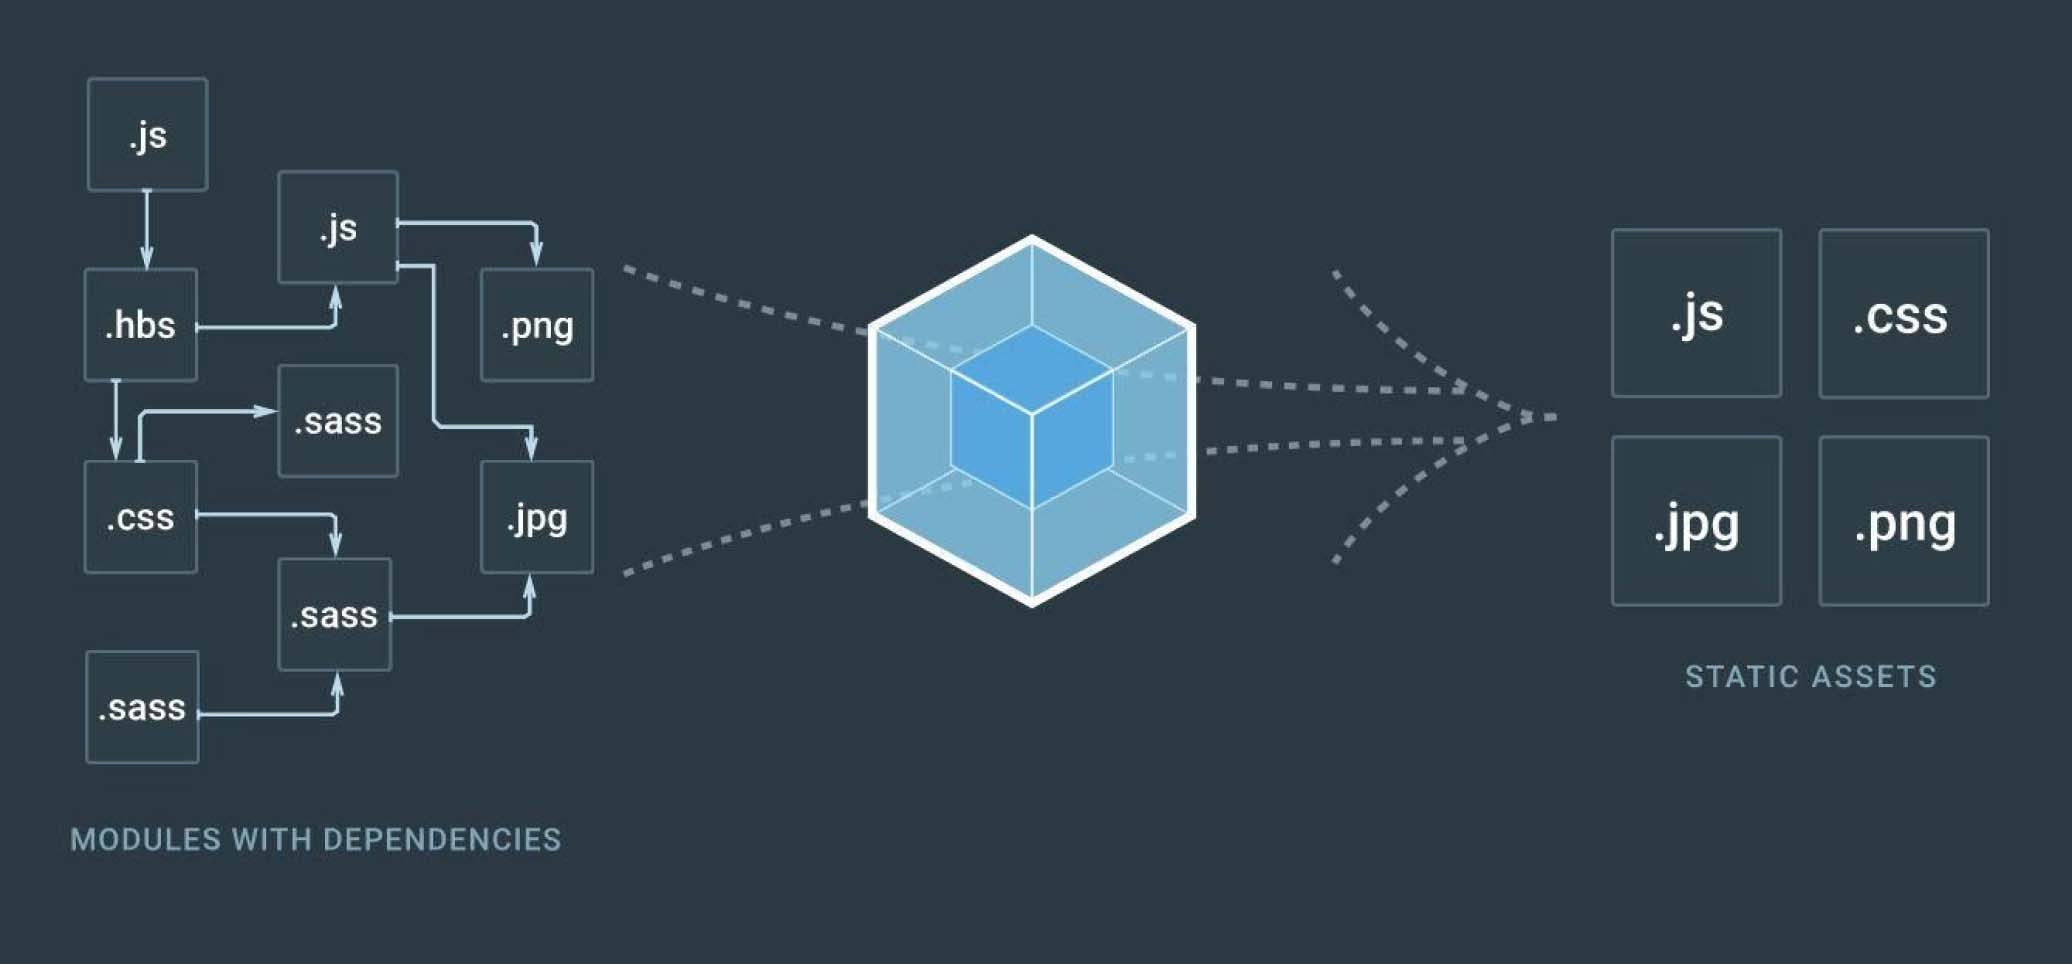
\includegraphics{Webpack}

\subsubsection{Rollup and Parcel}
...
\subsection{Unbundled development}

The examples we looked at so far are all module bundlers that use the concepts of bundled development. One very important thing to note is the word development. The differences between both approaches lies only in the development phase. The advantages of unbundled development are only noticeable when the developer or the development team is actually developing the application. When it is time to make a production build that the end-user will be able to use, the following unbundled development build tools still use the same module bundlers discussed in the previous section. So in essence, we can’t call the unbundled development build tools module bundlers, because they don’t bundle anything. They do use module bundlers.

Because most browsers now support ESM, bundling all Javascript modules of a project into one output file isn’t necessary. All non-Javascript modules do have to be translated or built to a valid Javascript module using a built tool (in WebPack this is called a Loader). In bundled development, when the development server is started, the whole project first has to be built and bundled; When a file is changed that file is rebuilt and then the whole project is again rebundled. In unbundled development a file is only built when it’s requested, meaning very fast startup time of the server. When a file is built, it is cached indefinitely. The browser will never have to download a file twice until it changes. When a file does change, only that single file has to be rebuilt. 

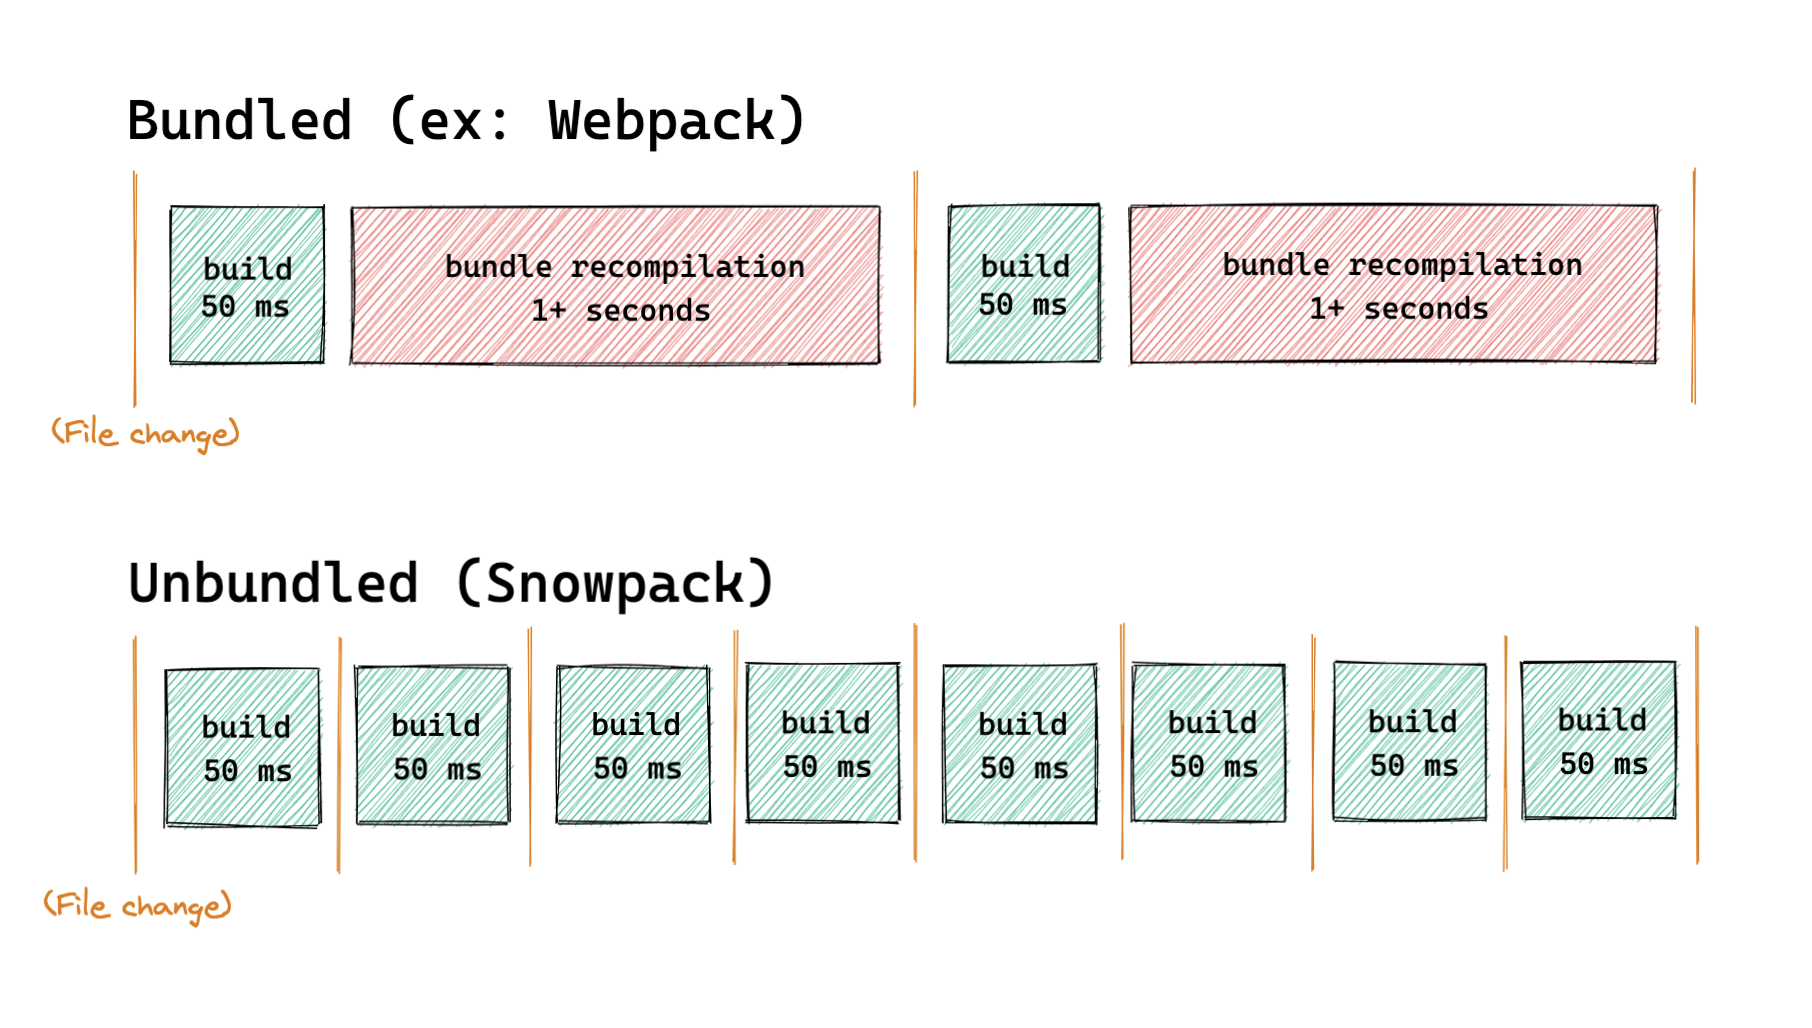
\includegraphics[scale=0.6]{Bundledvsunbundled}

All this results in very fast development performance compared to bundled development tools like WebPack. However, as mentioned before, unbundled development tools still use traditional module bundlers to make a production build. It does this because the advantages of Tree-shaking, a single output file and other features of module bundlers still hold up in the production phase: Tree-shaking results in a smaller output file; importing non-Javascript or CommonJS modules into ESMs is not supported in browsers; Not all modules are written with ESM; and the list goes on. We’ll now look at two examples of unbundled development tools.

\subsubsection{Snowpack}
...
\subsubsection{Vite}
...
